\section{Theorie}
\label{sec:Theorie}

\subsection{Allgemeine Brückenschaltung}

\begin{figure}
    \centering
    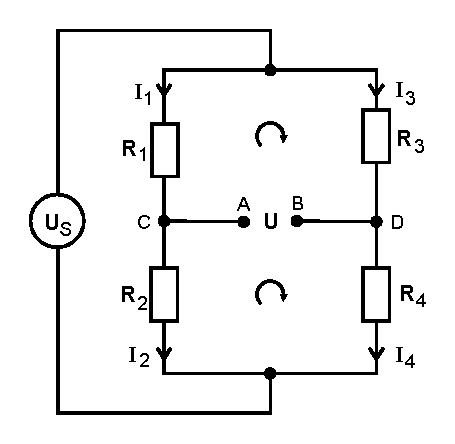
\includegraphics[width=0.5\textwidth]{pictures/schaltung1.pdf}
    \caption{Ein beispielhafter Aufbau einer einfachen Brückenschaltung \cite[1]{v302}.}
    \label{fig:Schaltung1}
\end{figure}

Brückenschaltungen sind essentiell, wenn unbekannte Widerstände bestimmt werden sollen.
Um mit einer Brückenschaltung, beispielsweise wie in Abbildung \ref{fig:Schaltung1},
benötigt man eine bakannte Speisespannung $U_\text{S}$ und vier Widerstände.
Durch alle Widerstände wird ein Strom fließen.
Es gelten die \textit{Kirchhoffschen Regeln}.
Es gilt für die Summe aller Ströme an einem Knotenpunkt
\begin{equation} \label{eq:kirch1}
    \sum_k I_k = 0 \, ,
\end{equation}
und für die Summe der Spannungen in einem abgeschlossenen Stromkreis
\begin{equation} \label{eq:kirch2}
    \sum_k U_k = 0 \, .
\end{equation}

Durch diese Regeln lässt sich die Formel für die Brückenspannung, die an den Punkten $A$ und $B$ abgegriffen wird,
angeben. Diese lautet
\begin{equation}
    U_\text{Brück} = \frac {R_2 R_3 - R_1 R_4} {(R_3 + R_4)(R_1 + R_2)} U_\text{S} \, .
\end{equation}

Es kann durchaus der Fall auftreten, oder willentlich bewirkt werden, dass die Brückenspannung vollständig verschwindet.
In diesem Falle gilt
\begin{equation} \label{eq:Brückenspannunggleich0}
    R_2 R_3 = R_1 R_4 \, .
\end{equation}

\subsection{Wheatstonesche Brücke}

\begin{figure}
    \centering
    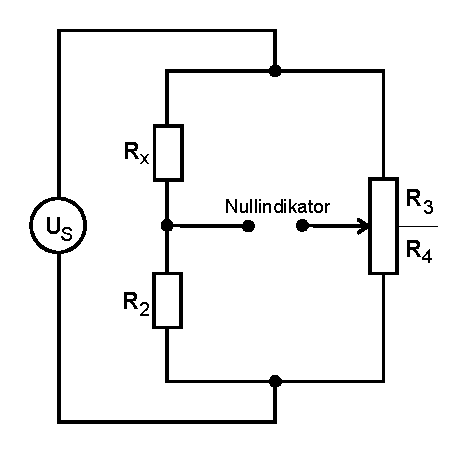
\includegraphics[width=0.5\textwidth]{pictures/schaltung2.pdf}
    \caption{Die Wheatstonesche Brückenschaltung \cite[4]{v302}.}
    \label{fig:Schaltung2}
\end{figure}

Mit der Wheatstonschen Brückenschaltung lassen sich besonders einfach unbekannte ohmsche Widerstände bestimmen.
Die Schaltung ist analog zu der in Abbildung \ref{fig:Schaltung1}, mit der Ausnahme das $R_1$ nun durch einen unbekannten Widerstand
$R_x$ ersetzt wird.
Durch die Gleichung (\ref{eq:Brückenspannunggleich0}) erhält man dann 
\begin{equation} \label{eq:Rx}
    R_x = \frac {R_2 R_3}{R_4} \, .
\end{equation}
Anstelle von $R_3$ und $R_4$ kann ebenfalls ein Potentiometer benutzt werden.

\subsection{Kapazitätsmessbrücke}

\begin{figure}
    \centering
    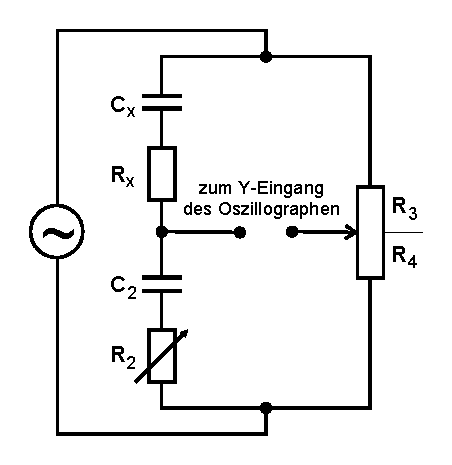
\includegraphics[width=0.5\textwidth]{pictures/schaltung3.pdf}
    \caption{Eine Kapazitätmessbrücke mit unbekanntem ohmschen und kapazitiven Widerstand \cite[5]{v302}.}
    \label{fig:Schaltung3}
\end{figure}

Mit der Kapazitätsmessbrücke lassen sich komplexe Widerstände bestimmen. 
Ein realer Kondensator ist aber niemals rein kapazitiv, sondern immer auch teilweise ohmisch.
Das bedeutet, der Widerstand wird über eine Reihenschaltung wie in Abbildung \ref{fig:Schaltung3} realisiert.
Natürlich muss bei dieser Art Widerstand Wechselstrom angelegt werden, da sonst der Kondensator eine Art 
unendlich großer Widerstand wird und der Zweck der Messung verfehlt wird.
Für diese Schaltung gelten die Gleichungen
\begin{align} \label{eq:Cx}
    C_x &= C_2 \frac {R_4}{R_3} & \text{und} & &   R_x = R_2 \frac {R_3}{R_4} \, .
\end{align}

\subsection{Induktivitätsmessbrücke}

\begin{figure}
    \centering
    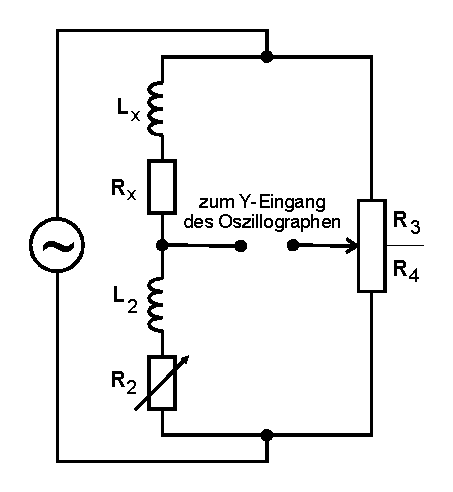
\includegraphics[width=0.5\textwidth]{pictures/schaltung4.pdf}
    \caption{Die Induktivitätsmessbrücke mit unbekanntem ohmschen und induktiven Widerstand \cite[6]{v302}.}
    \label{fig:Schaltung4}
\end{figure}

Mit einer Induktivitätsmessbrücke werden nun Induktivitäten gemessen.
Auch diese komplexen Widerstände bestehen immer aus einem ohmschen und einem induktiven Widerstand.
Diese werden dann im Schaltbild dadurch realisiert, dass sie in Reihe geschalten werden.
Das vollständige Schaltbild ist in Abbildung \ref{fig:Schaltung4} zu sehen.
Für die unbekannten Induktivitäten ergibt sich
\begin{equation} \label{eq:L_x}
    L_x = L_2 \frac{R_3}{R_4}
\end{equation}
und für den ohmschen Widerstand des Widerstandes
\begin{equation} \label{eq:induktR_x}
    R_x = R_2 \frac{R_3}{R_4}
\end{equation}

\subsection{Maxwell Brücke}
\begin{figure}
    \centering
    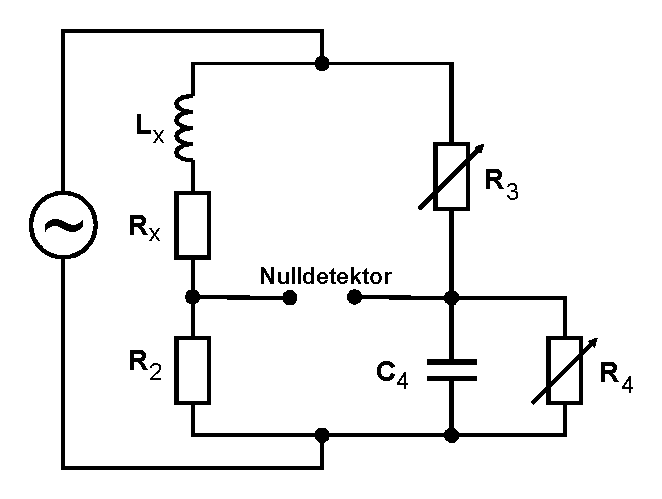
\includegraphics[width=0.5\textwidth]{pictures/schaltung5.pdf}
    \caption{Eine Maxwellsche Brückenschaltung zur Messung eines ohmschen und induktiven Widerstandes \cite[7]{v302}.}
    \label{fig:Schaltung5}
\end{figure}

Eine alternative zu der Induktivitätsmessbrücke ist die Maxwellbrücke.
Auch diese Brückenschaltung ist eine Schaltung, um Induktivitäten zu bestimmen.
Der grundlegende Unterschied liegt darin, dass ein Bauteil ausgetauscht wird.
Dabei handelt es sich um die bekannte Induktivität $L_2$.
Nun wird eine bekannte Kapazität benötigt.
Diese hat baubedingt einen deutlich geringeren ohmschen Widerstand.
Nun werden die Unbekannten durch die Gleichungen
\begin{equation} \label{eq:maxwL_x}
    L_x = R_2 R_3 C_4
\end{equation}
und 
\begin{equation} \label{eq:maxwR_x}
    R_x = R_2 \frac{R_3}{R_4}
\end{equation}
beschrieben.

\subsection{Wien-Robinson-Brücke}

\begin{figure}
    \centering
    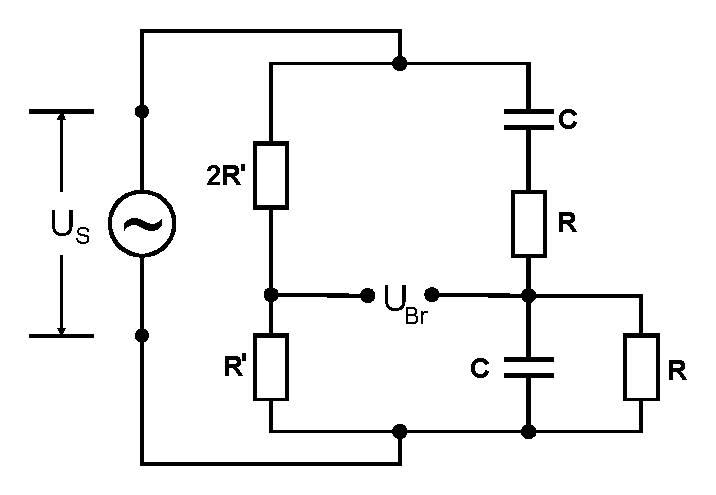
\includegraphics[width=0.5\textwidth]{pictures/schaltung6.pdf}
    \caption{Die Wien-Robinson-Brücke \cite[8]{v302}.}
    \label{fig:Schaltung6}
\end{figure}

Die Wien-Robinson-Brücke, dargestellt in Abbildung \ref{fig:Schaltung6}, ist eine Brückenschaltung
die vor allem als Bandpass funktionert. 
Ein Bandpass ist ein elektronischer Filter, der  nur bestimmte Frequenzbänder hindurch lässt.
Die Formel
\begin{equation} \label{eq:Wien1}
    \left|\frac{U_\text{Br}}{U_\text{S}}\right|^2 =  \frac{\left({\omega}^2 R^2 C^2 -1 \right)^2}
    {9 \left[ \left( 1 - {\omega}^2 R^2 C^2 \right)^2 + 9 {\omega}^2 R^2 C^2 \right]}
\end{equation}
sei hier nur angegeben \cite[9]{v302}.
Jedoch wird hier erkennbar, dass die Brückenspannung dann verschwindet, wenn
\begin{equation*}
    \omega_0 = \frac{1}{R C}
\end{equation*}
gilt. Nun kann man sich das Frequenzverhältnis definieren als
\begin{equation*}
    \Omega \coloneq \frac{\nu}{\nu_0} \quad \text{mit} \quad \nu_0 = \frac{\omega_0}{2\pi} \, .
\end{equation*}
Führt man $\Omega$ in (\ref{eq:Wien1}) ein, verändert sich die Gleichung zu der Form
\begin{equation} \label{eq:Wien2}
    \left|\frac{U_\text{Br}}{U_\text{S}}\right|^2 = \frac{\left( \Omega^2 -1 \right)^2}
    {9 \left( \left( 1 - \Omega^2 \right)^2 + 9 \Omega^2 \right)}
\end{equation}
Mit der Wien-Robinson-Brücke lässt sich eine sogenannte Klirrfaktor-Messung durchführen.
Das bedeutet, dass der Anteil an Oberwellen im Verhältnis zur Grundwelle eines Generators gemessen wird.
Ein Sinusgenerator sollte beispielsweise keine Oberwellen haben.
Ist der Klirrfaktor also klein, ist die Qualität des Sinusgeneratores hoch.
Der Klierfaktor ist gegeben durch
\begin{equation} \label{eq:klirr}
    k \coloneq \frac {\sum_{i=2}^{N} {U_i}^2}{U_1}  \, .
\end{equation}